\documentclass[12pt]{article}
\usepackage{amsmath}
\usepackage{amssymb}
\usepackage{fancyhdr}
\usepackage{geometry}
\usepackage{hanging}
\usepackage{enumitem}
\usepackage{graphicx}
\usepackage{setspace}
\usepackage{tabularx}
\usepackage{array}
\usepackage[table]{xcolor}
\usepackage{longtable}
\usepackage{booktabs}
\usepackage[colorlinks=true, linkcolor=blue]{hyperref}
\usepackage{parskip}
\usepackage{listings}
\usepackage{mdframed}
\usepackage{pifont}
\usepackage{tikz}
\usepackage{tikzpagenodes}
%\usepackage{lipsum} %remove later
\doublespacing
%\setlength\parindent{28 pt}
\geometry{letterpaper, margin=1in}

% ++++ Color definitions ++++
\definecolor{highcol}{HTML}{C00000}
\definecolor{medcol}{HTML}{BF8F00}
\definecolor{lowcol}{HTML}{375623}
\definecolor{immediatecol}{HTML}{C00000}
\definecolor{shortcol}{HTML}{E26B0A}
\definecolor{longcol}{HTML}{375623}
\definecolor{headercol}{HTML}{1F4E79}
\definecolor{lightyellow}{HTML}{FFF2CC}
\definecolor{lightgreen}{HTML}{EBF1DD}
\definecolor{lightred}{HTML}{FFD7D7}
\definecolor{lightgray}{HTML}{EDEDED}
\definecolor{codebg}{HTML}{F5F5F5}
\definecolor{codeframe}{HTML}{CCCCCC}
\definecolor{impactbg}{HTML}{FFF2CC}
\definecolor{impactframe}{HTML}{BF8F00}
\definecolor{verifybg}{HTML}{EBF1DD}
\definecolor{verifyframe}{HTML}{375623}
\definecolor{warnbg}{HTML}{FFD7D7}
\definecolor{warnframe}{HTML}{C00000}
\definecolor{notebg}{HTML}{DDEEFF}
\definecolor{noteframe}{HTML}{1F4E79}
\definecolor{checkbg}{HTML}{F2F2F2}
\definecolor{checkframe}{HTML}{595959}
\definecolor{acccol}{HTML}{1F4E79}
\definecolor{transcol}{HTML}{375623}
\definecolor{integcol}{HTML}{7030A0}
\definecolor{authcol}{HTML}{C00000}
\definecolor{immediatecol}{HTML}{C00000}
\definecolor{shortcol}{HTML}{E26B0A}
\definecolor{longcol}{HTML}{375623}
\definecolor{totalrowcol}{HTML}{D9E1F2}
\definecolor{subtotalcol}{HTML}{F2F2F2}
 

% ++++ Convenience macros ++++
% Severity badge: \sevbadge{colour}{label}
\newcommand{\sevbadge}[2]{%
  \colorbox{#1}{\color{white}\textbf{\small #2}}%
}
 
% Timeframe badge
\newcommand{\tfbadge}[2]{%
  \colorbox{#1}{\color{white}\textbf{\small #2}}%
}
 
% Header row cell (white text on dark blue)
\newcommand{\hcell}[1]{%
  \cellcolor{headercol}\color{white}\textbf{#1}%
}

\newcommand{\sectionrule}{%
  \vspace{4pt}\noindent\textcolor{headercol}{\rule{\linewidth}{0.8pt}}\vspace{4pt}%
}

\newcommand{\hipbadge}[2]{%
  \colorbox{#1}{\color{white}\textbf{\small #2}}%
}

% Checkbox item
\newcommand{\cbox}{\ding{113}\;}

% ── Listings style (terminal / config blocks) ────────────────────────────
\lstdefinestyle{terminal}{
  backgroundcolor=\color{codebg},
  basicstyle=\ttfamily\small,
  breaklines=true,
  breakatwhitespace=false,
  frame=single,
  rulecolor=\color{codeframe},
  xleftmargin=8pt,
  xrightmargin=8pt,
  aboveskip=6pt,
  belowskip=6pt,
  showstringspaces=false,
  columns=fullflexible,
  keepspaces=true,
}
 
% ── Framed boxes ─────────────────────────────────────────────────────────
\newmdenv[
  backgroundcolor=impactbg,
  linecolor=impactframe,
  linewidth=1.2pt,
  innerleftmargin=8pt,
  innerrightmargin=8pt,
  innertopmargin=6pt,
  innerbottommargin=6pt,
  skipabove=6pt,
  skipbelow=6pt,
]{impactbox}
 
\newmdenv[
  backgroundcolor=verifybg,
  linecolor=verifyframe,
  linewidth=1.2pt,
  innerleftmargin=8pt,
  innerrightmargin=8pt,
  innertopmargin=6pt,
  innerbottommargin=6pt,
  skipabove=6pt,
  skipbelow=6pt,
]{verifybox}
 
\newmdenv[
  backgroundcolor=warnbg,
  linecolor=warnframe,
  linewidth=1.2pt,
  innerleftmargin=8pt,
  innerrightmargin=8pt,
  innertopmargin=6pt,
  innerbottommargin=6pt,
  skipabove=6pt,
  skipbelow=6pt,
]{warnbox}

\newmdenv[
  backgroundcolor=notebg,
  linecolor=noteframe,
  linewidth=1.2pt,
  innerleftmargin=8pt,
  innerrightmargin=8pt,
  innertopmargin=6pt,
  innerbottommargin=6pt,
  skipabove=6pt,
  skipbelow=6pt,
]{notebox}

\newmdenv[
  backgroundcolor=checkbg,
  linecolor=checkframe,
  linewidth=1.2pt,
  innerleftmargin=8pt,
  innerrightmargin=8pt,
  innertopmargin=6pt,
  innerbottommargin=6pt,
  skipabove=6pt,
  skipbelow=6pt,
]{checklistbox}

% ++++ Fancy Settings (for header) ++++
\pagestyle{plain}
\fancypagestyle{main}{
	\fancyhf{}
	\lhead{Malware Analysis}
	\rhead{\leftmark}
	\cfoot{\thepage}
	\renewcommand{\headrulewidth}{0.4pt}
}

% Column widths (tweak the numbers if you want)
\newcommand{\colNum}{0.06\linewidth}   % column 1 (1–10)
\newcommand{\colSmall}{0.16\linewidth} % columns 2,3,5
\newcommand{\colBig}{0.48\linewidth}   % column 4 (3x colSmall)

% ++++ Begin Doc ++++

\begin{document}

% ++++ Cover Page ++++

\begin{titlepage}
\begin{tikzpicture}[remember picture, overlay]
  \draw[line width=1pt]
    ([shift={(1in,-1in)}]current page.north west)
    rectangle
    ([shift={(-1in,1in)}]current page.south east);
\end{tikzpicture}
\centering
\vfill

% ++Logo

\includegraphics[width=0.35\textwidth]{images/logo.png}

\vspace{1.5cm}

% ++Title
\LARGE{\textbf{Lab 11: Malware Analysis}}\\
\vspace{0.3cm}
\large{\textbf{Keith Schoen}}\\
\vspace{0.3cm}
\large{\textbf{CSEC3755-001}}\\
\vspace{0.3cm}
\large{\textbf{Dr. Daniel Pittman}}\\
\vspace{0.3cm}
\large{\textbf{30 April 2026}}\\
\vspace{0.3cm}

\vfill
\end{titlepage}

% ++++ ToC ++++

\pagenumbering{gobble} %hide page numbers for cover and ToC
\tableofcontents
\clearpage

% ++++ Begin Report ++++

\pagenumbering{arabic} %page one starts here
\setcounter{page}{1}
\pagestyle{main} %turn on fancy

% ++++ Executive Summary ++++
\section{Executive Summary}

% ++++ Part01 Triage & File Identification
\section{Triage \& File Identification}
\smallskip
\begin{notebox}
\textbf{Note about this section:}\\
The \texttt{Add-WindowsCapability} command for Sysmon that 
was given did not work for this environment. Instead, I used the following:
\begin{lstlisting}[style=terminal]
# Download
Invoke-WebRequest -Uri "https://download.sysinternals.com/files/Sysmon.zip" -OutFile "$env:TEMP\Sysmon.zip"

# Extract
Expand-Archive -Path "$env:TEMP\Sysmon.zip" -DestinationPath "C:\Tools\Sysmon"

# Install (run this as Admin)
C:\Tools\Sysmon\Sysmon64.exe -accepteula -i
\end{lstlisting}
\end{notebox}
\bigskip
\subsection{Creating the EICAR Test File (Sample A)}
The following screenshots show the process of creating the EICAR test
file in the Windows VM. I used the full sting given hoping to see 
Defender defy my expectations and catch the file at creation, but the 
file survived create and \texttt{Get-Content}
\smallskip
\begin{center}
	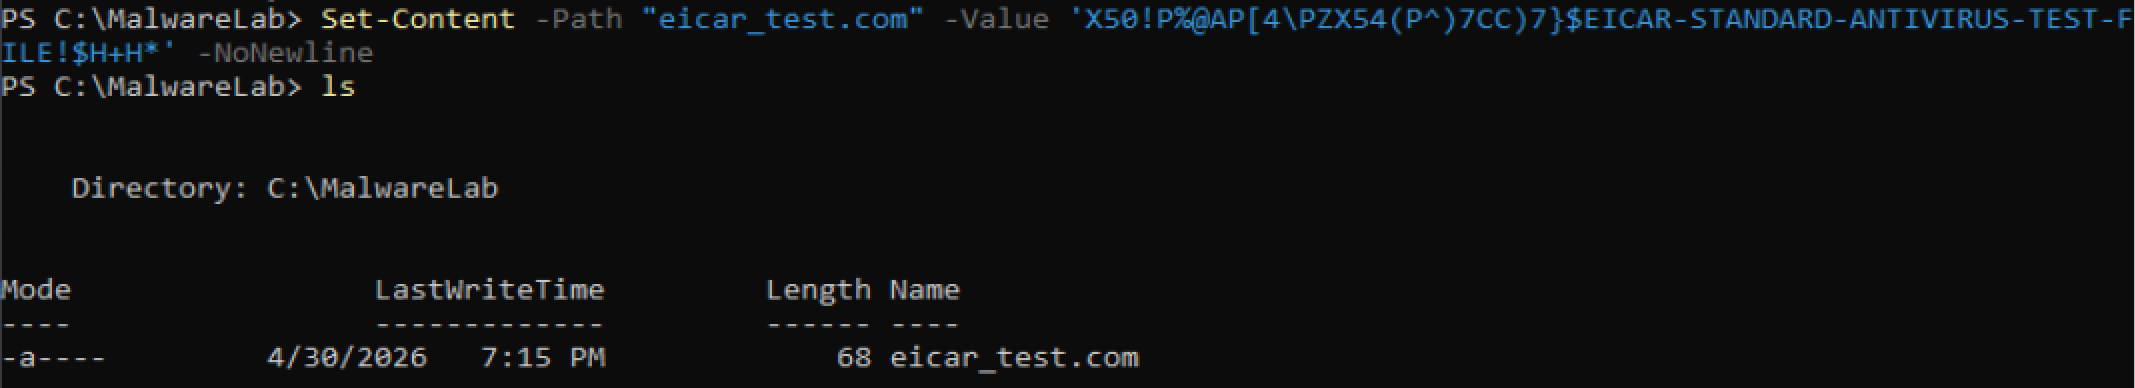
\includegraphics[width=0.75\textwidth]{images/1.1-eicarcreated.png}\\ 
	\textit{Figure 1.1: Creation of the EICAR test file}
\end{center}
\smallskip
\begin{center}
	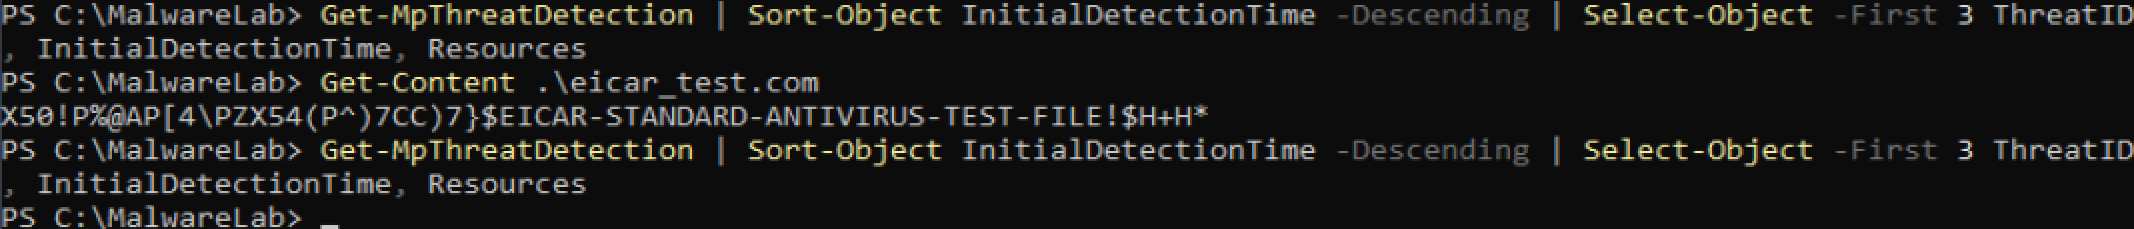
\includegraphics[width=0.75\textwidth]{images/1.2-nodefender.png}\\ 
	\textit{Figure 1.2: The EICAR test file survives Windows Defender}
\end{center}
\smallskip
\subsection{Basic File Identification}
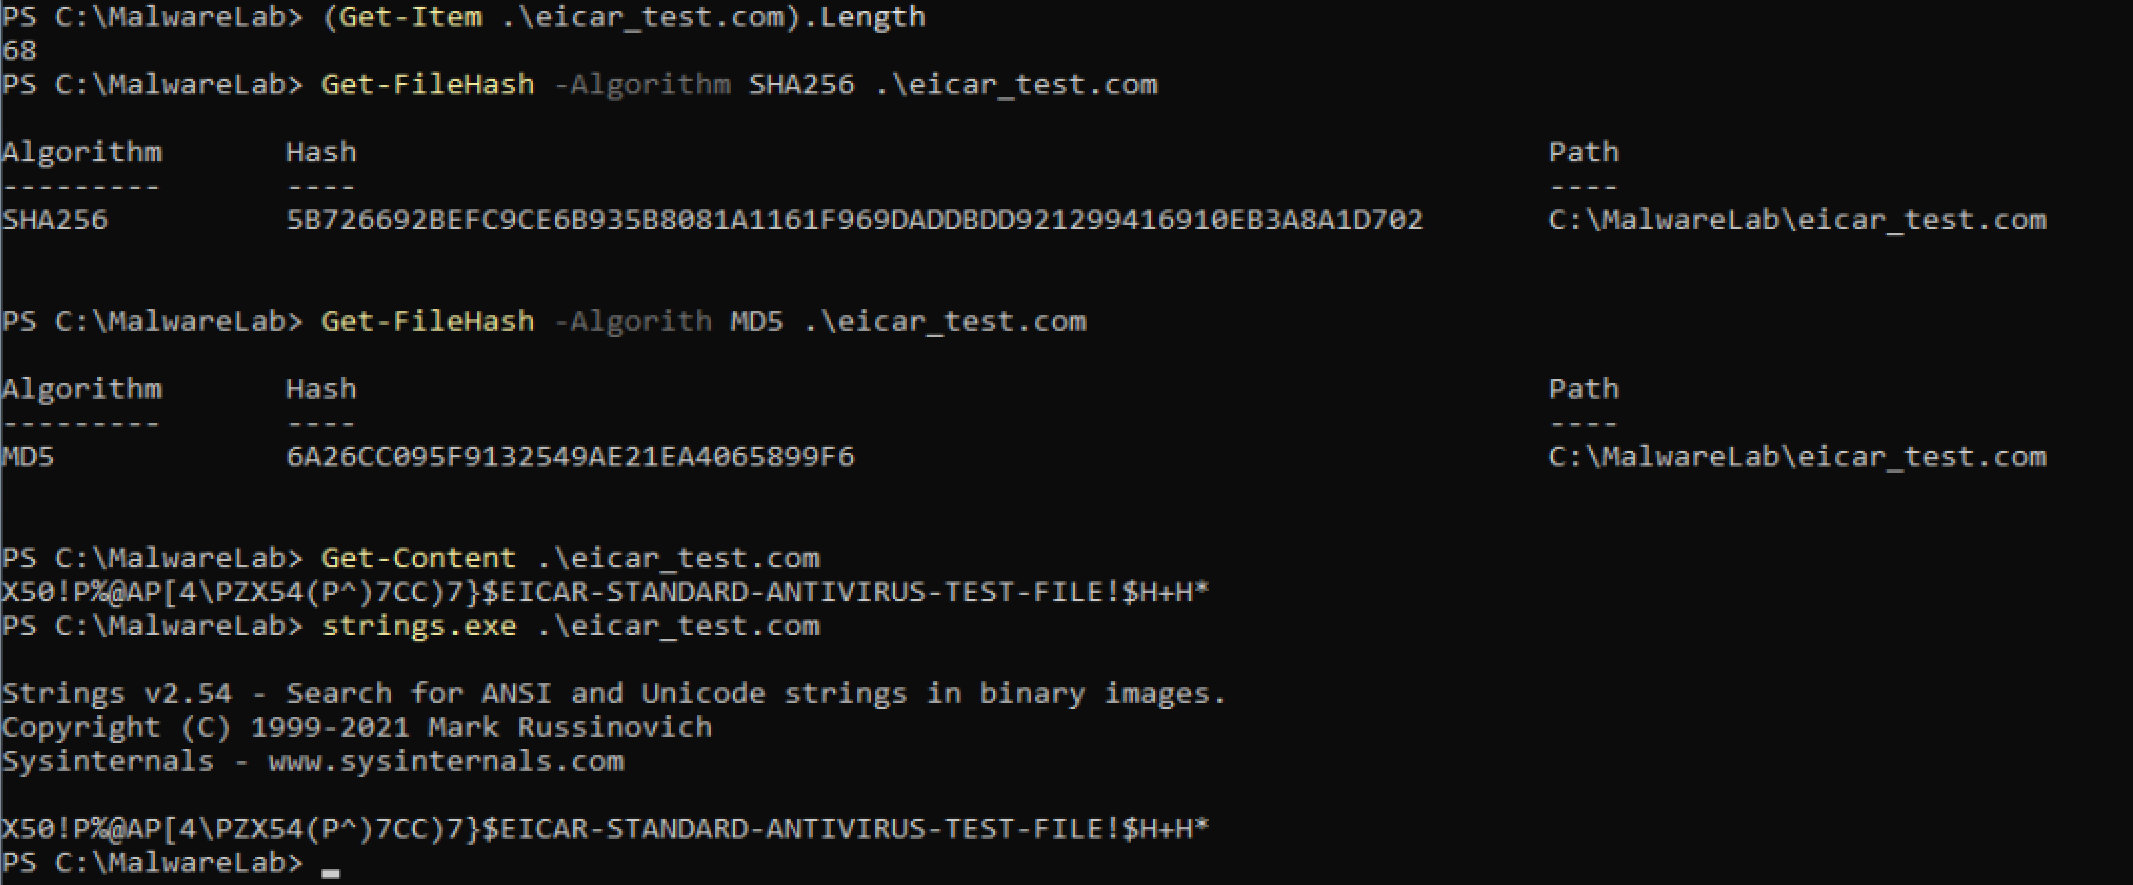
\includegraphics[width=\textwidth]{images/1.3-fileidentification.png}\\ 
\textit{Figure 1.3: Results of file identification commands for the EICAR test file}
\smallskip
\subsection{Hash Lookup on Virus Total}
\begin{itemize}
	\item Out of  62 security vendors on Virus Total, 6 flagged the file as malicious.
	\item A few names given for the threat are:
	\begin{itemize}
		\item \texttt{Virus/EICAR\underbar{   }Test\underbar{   }File}
		\item \texttt{NotAThreat.EICAR[TestFile]}
		\item \texttt{Eicar\underbar{   }test\underbar{   }1}
	\end{itemize}
	\item Tags shown for the 'threat' are:
	\begin{itemize}
		\item powershell
		\item idle
		\item long-sleeps
	\end{itemize}
	\item File type according to Virus Total: \textbf{Powershell}
	\item As for the community tab, there isn't any activity early then 10 years.
\end{itemize}
\smallskip
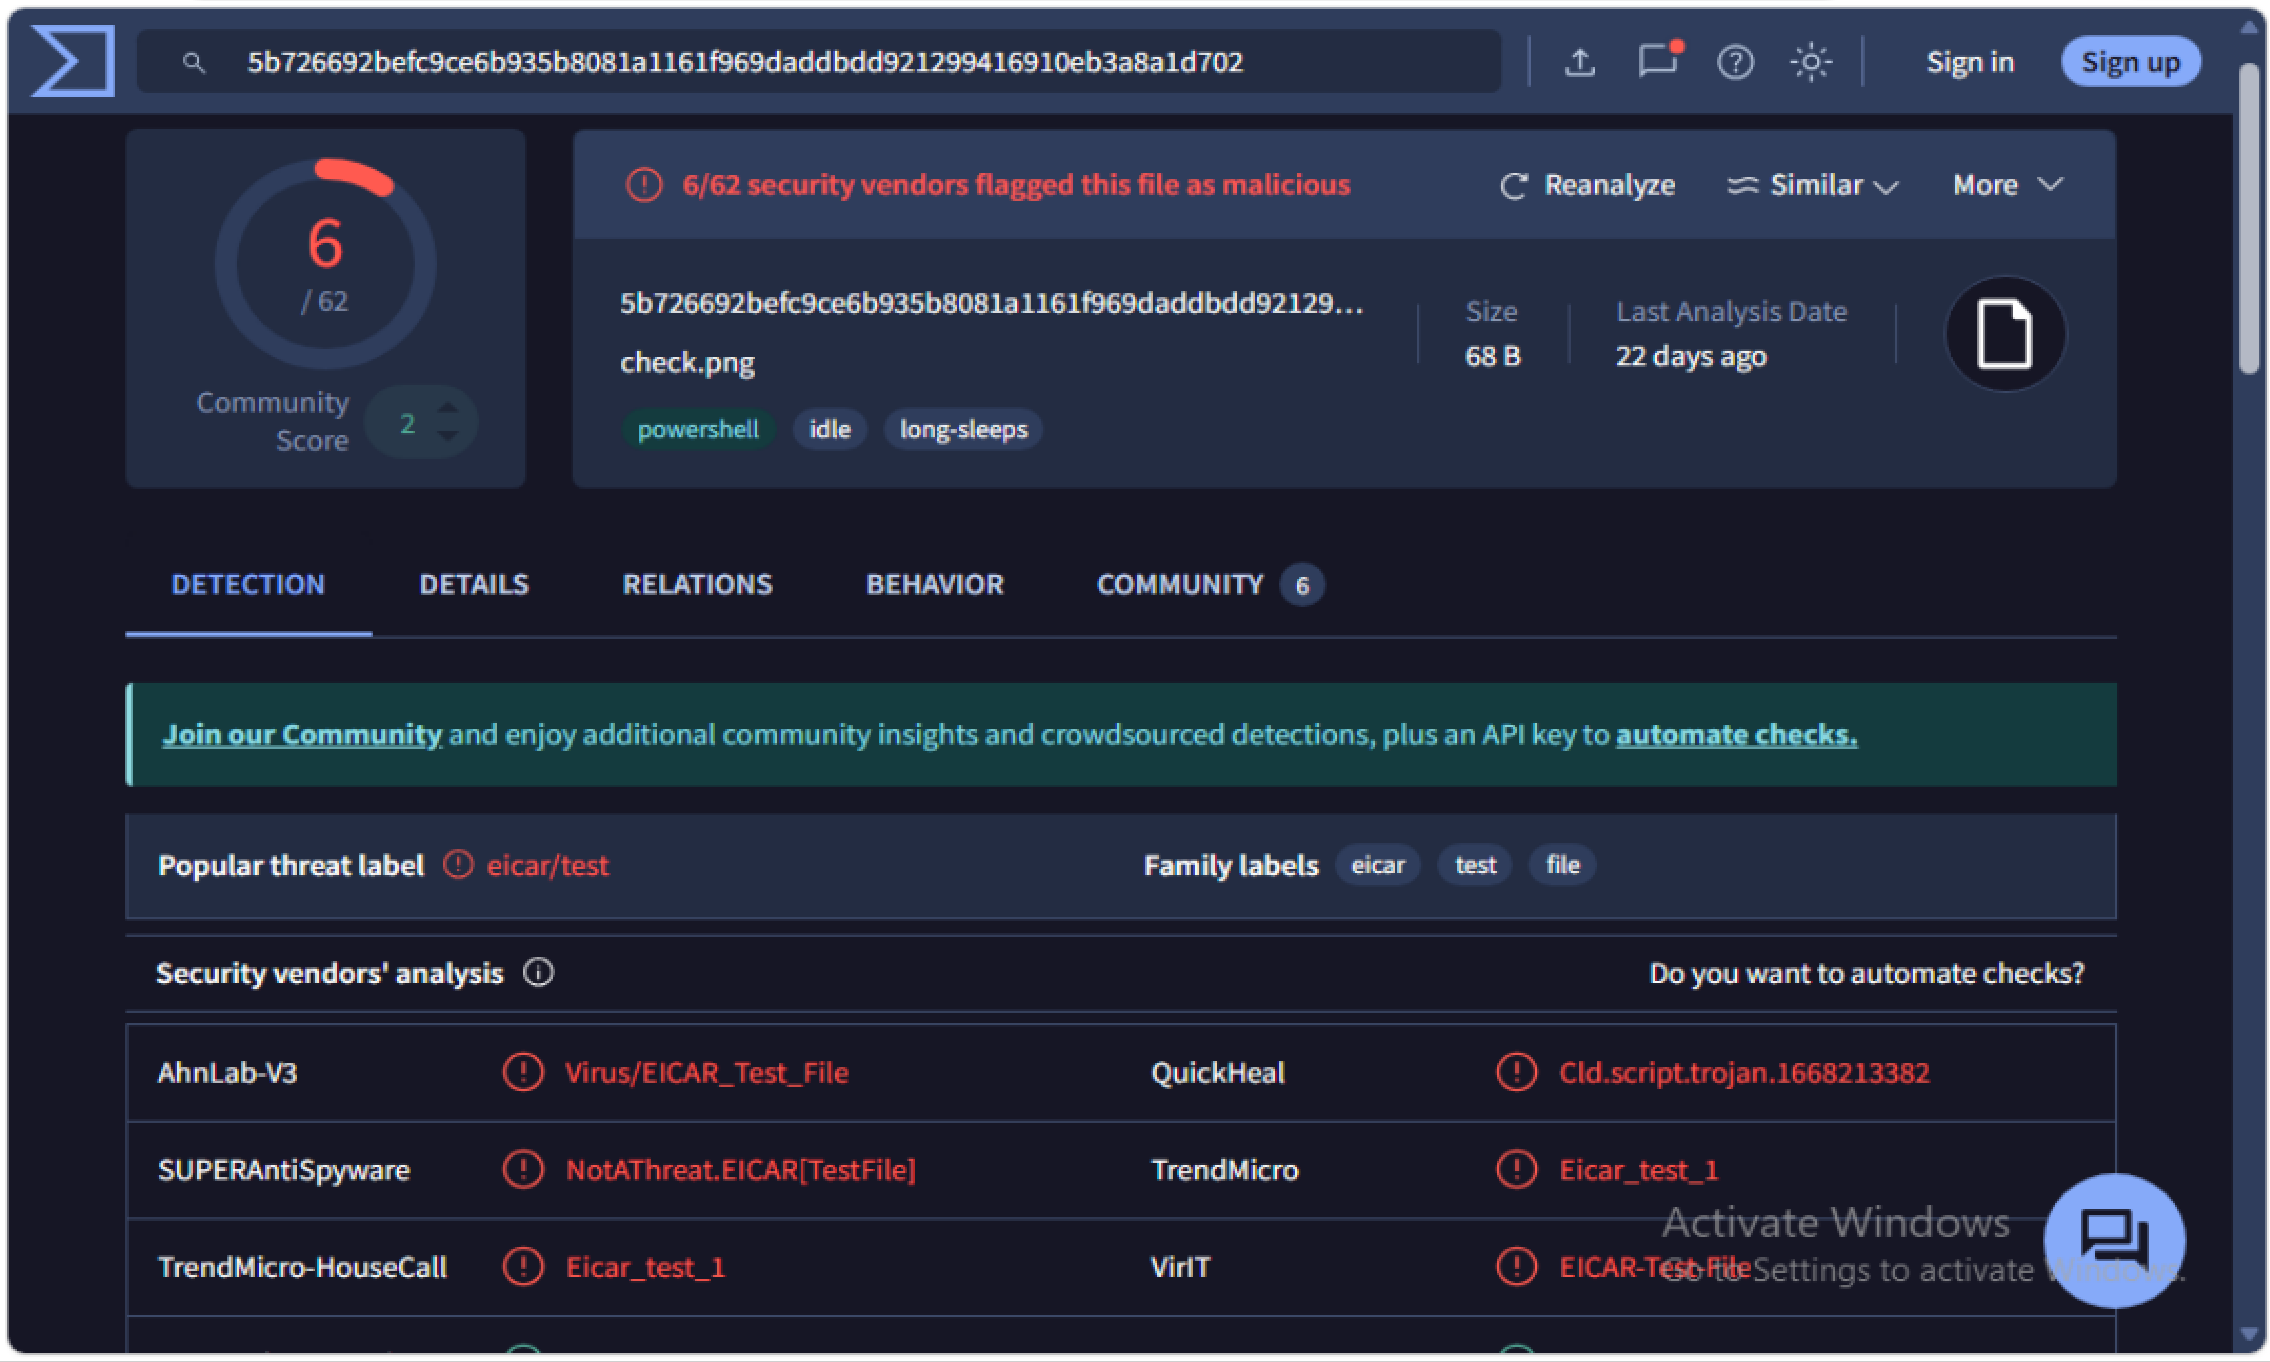
\includegraphics[width=\textwidth]{images/1.4-virustotaldock.png}\\
\textit{Figure 1.4: Results for Virus Total hash look-up}
\bigskip
\begin{notebox}
	It should be noted that while the results on Virus Total showed a 6/62, the only 
	results to show in the 'Security vendors' analysis' table were those from AhnLab-V3, 
	SUPERAntiSpyware, and TrendMicro-HouseCall.
\end{notebox}
\bigskip
\textbf{What kind of threat is this?}\\
This is an idle \textbf{Powershell script} that waits until the right conditions are met before
executing. This would explain how it was able to evade detection from Windows Defender 
despite being flagged as malicious.

% ++++ Part02 Static Analysis ++++
\section{Static Analysis}
\subsection{String Analysis with Sysinternals Strings}
Executed the following commands on the EICAR test file from section one to demonstrate 
how it works at a basic level:\\
\begin{lstlisting}[style=terminal]
	# Extract all strings at least 8 characters long and save to file
	strings.exe -n 8 .\eicar_test.com > eicar_strings.txt

	# Open the output and examine it
	notepad eicar_strings.txt
\end{lstlisting}
\bigskip
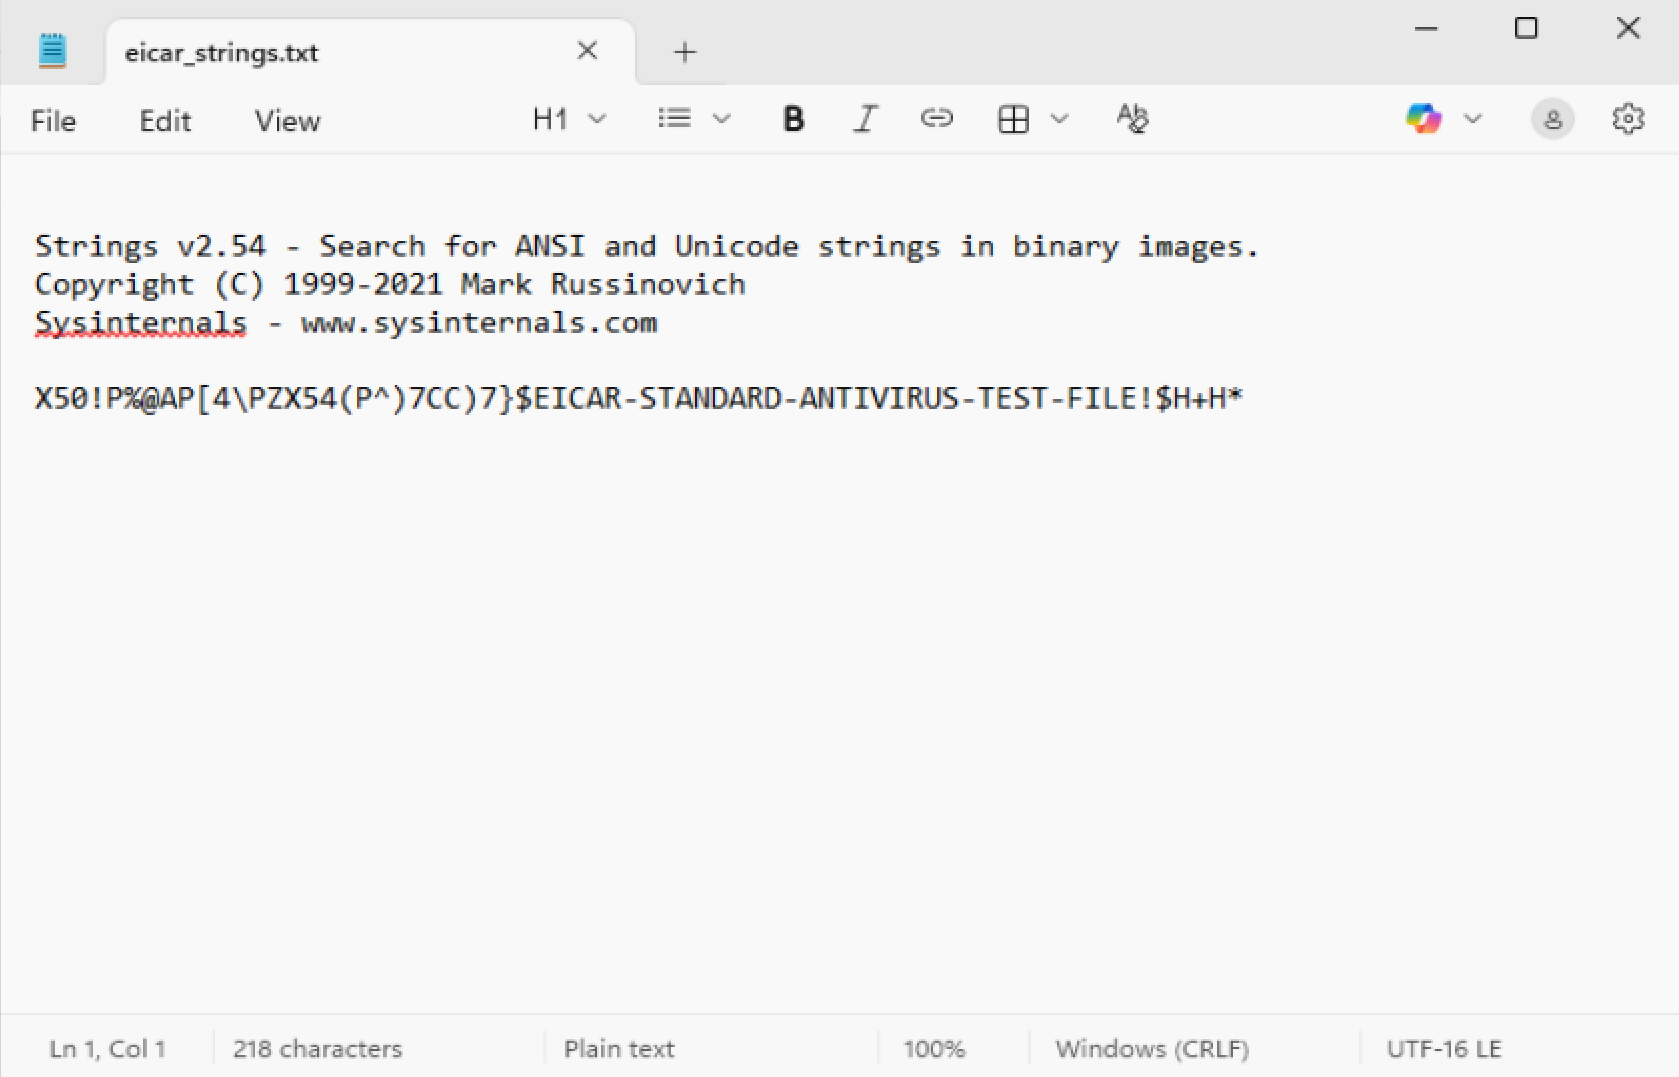
\includegraphics[width=\textwidth]{images/2.1-stringsoutput.png}\\
\textit{Figure 2.1: Strings output for the EICAR test file}
\subsection{Examine PE Structure via VirusTotal's Details Tab}
\bigskip
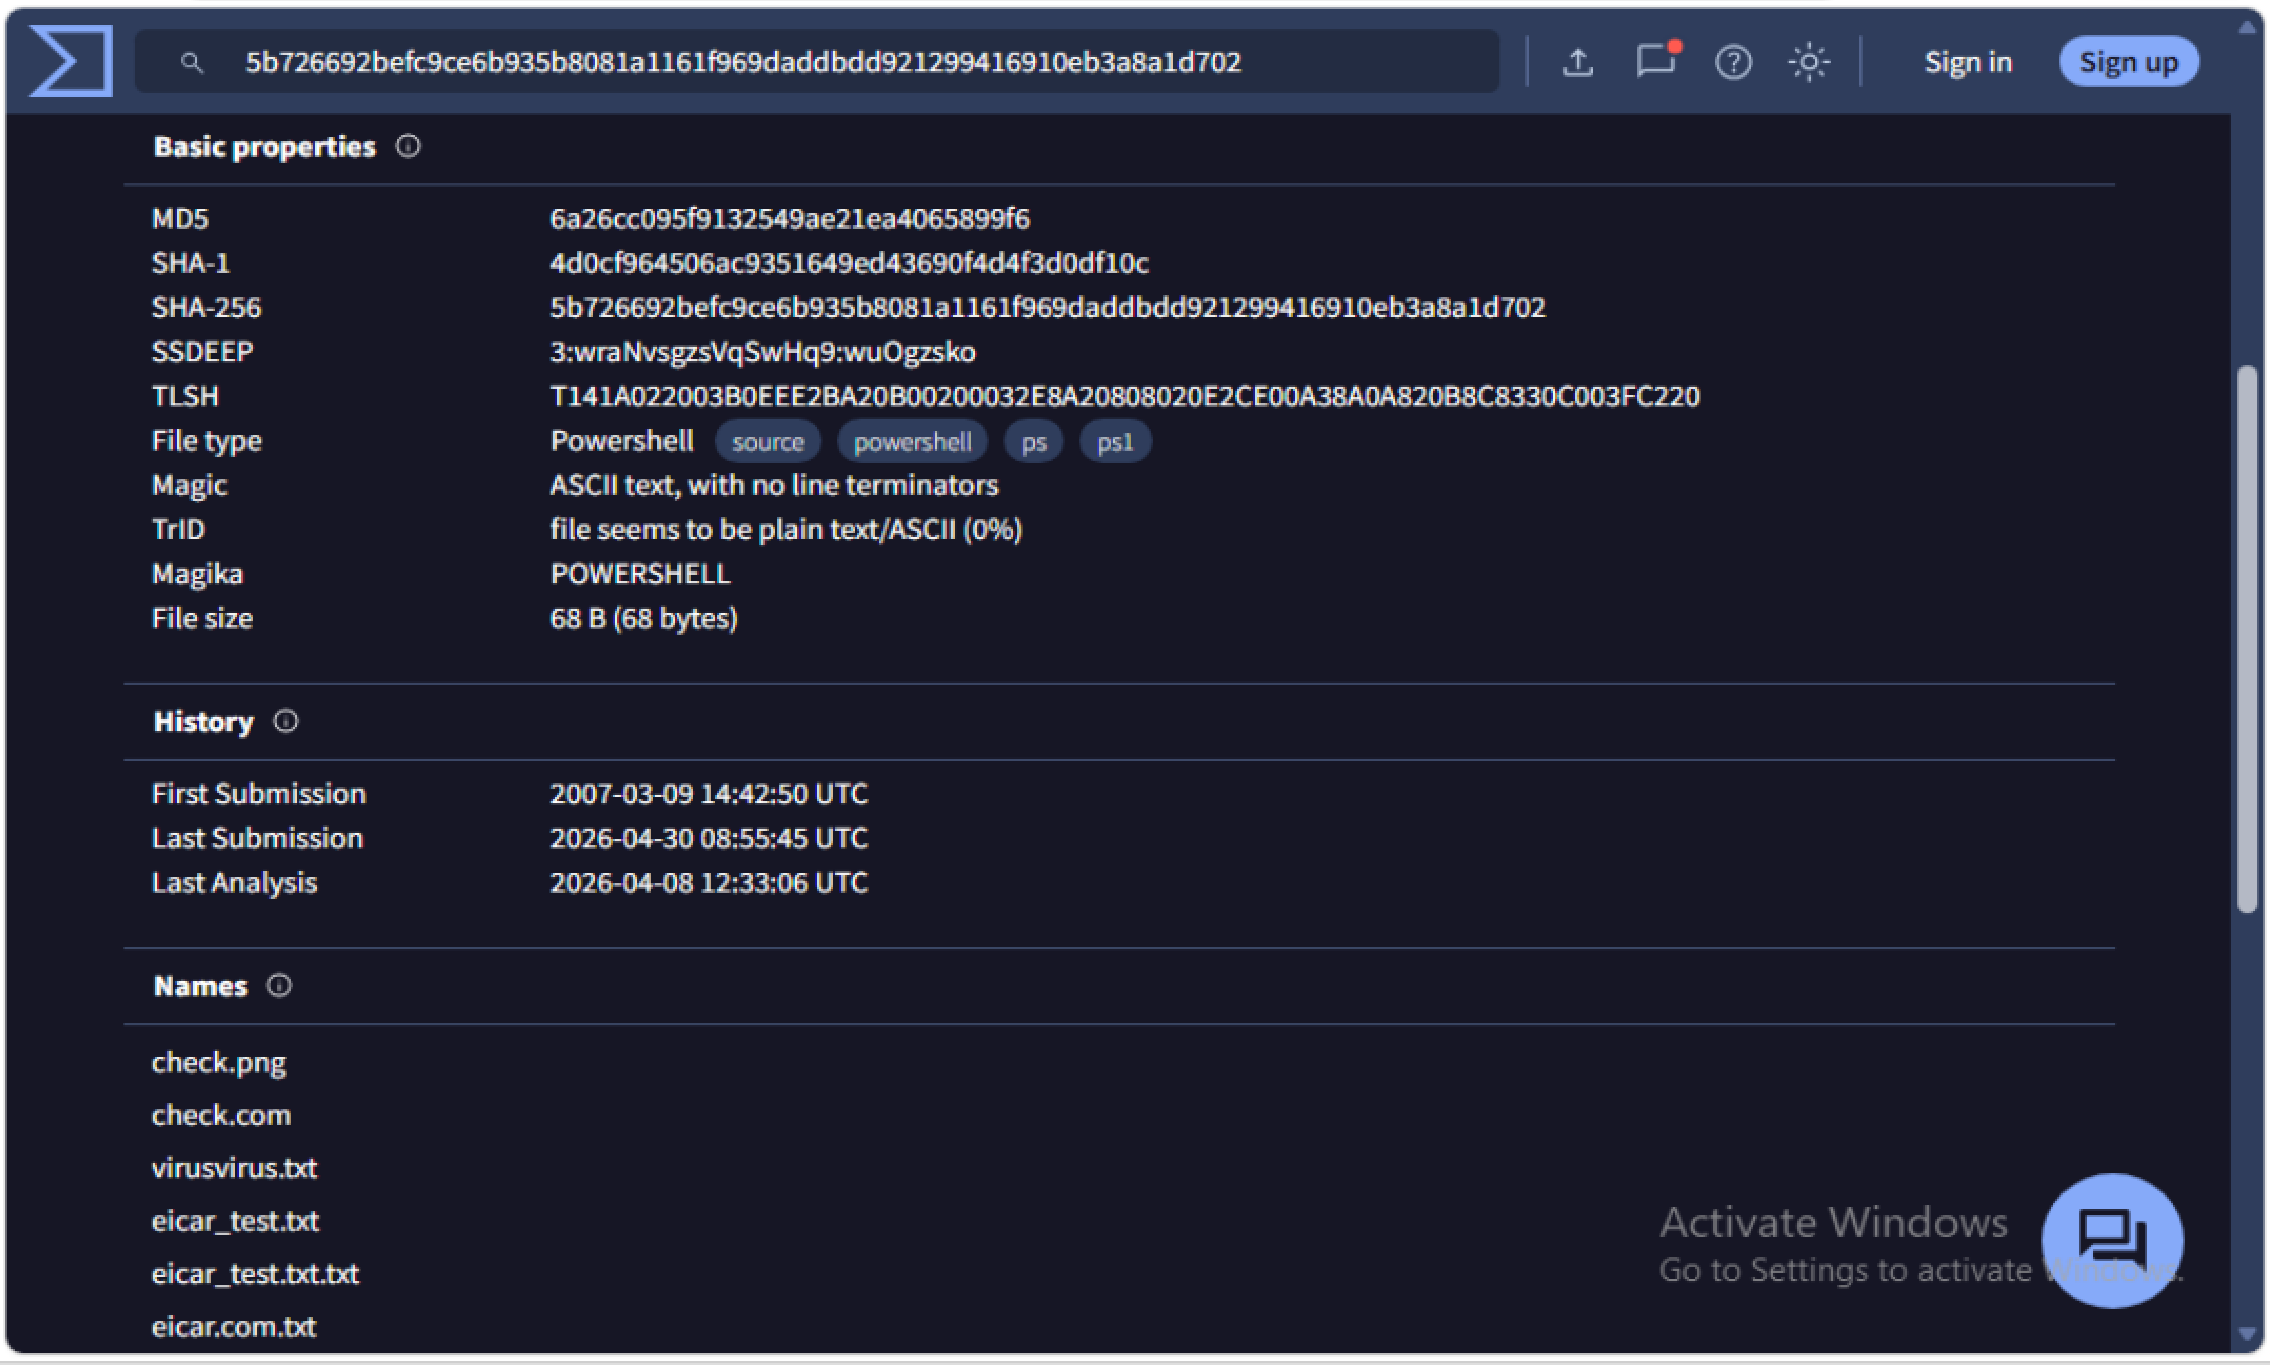
\includegraphics[width=\textwidth]{images/2.2-vtdetailseicar.png}\\
\textit{Figure2.2: Details section for EICAR test file hash lookup}
\subsection{Choose a Real Malware Sample (Sample B)}
\bigskip
\begin{warnbox}
\textbf{Note about malware selection for Sample B}\\
\textbf{SHA256 Hash:}939b247d1cf5a8b674ff632365af9982256363d6ae390876d0d3d9cbc07d163b\\
\textbf{Malware Family:} phantomstealer\\
\textbf{First submission to VT:} 2026-04-30 07:14:26 UTC\\
\textbf{VT Report URL:}\\
	https://www.virustotal.com/gui/file/939b247d1cf5a8b674ff632365af9982256363d6ae3908\\ 76d0d3d9cbc07d163b/summary\\
\textbf{Hybrid Analysis Report URL:}\\
	https://hybrid-analysis.com/sample/939b247d1cf5a8b674ff632365af9982256363d6ae39087\\ 6d0d3d9cbc07d163b/69f301586d9a87d56d06d3b7\\
\ \\
Honestly, I decided on a RAT because I like the animal and the malware category. When I did
quick overview, this one had tons of documentation making it an easy first grab. Along with
the amount of information already becoming available, it is made extra exciting in that this is
brand-new submission to VT (about 3 hours old). It's a great pick for Sample B.	
\end{warnbox}
\subsubsection{Exploring Sample B's Virus Total Page}
\textbf{Detection Tab}
\begin{itemize}
	\item \textbf{Detection Ratio:} 39/71
	\item This maleware is new so there isn't a name yet, but common themes include RAT, MSIL, 
	and Trojan. Skyhigh(SWG) seems to be the only AV that has given it a name so far: "Artemis!Trojan".
	The 'popular threat label' is \underbar{trojan.msil/phantomstealer}.
	\item \textbf{Family:} phantomstealer
\end{itemize}
\textbf{Details Tab}
\begin{itemize}
	\item \textbf{File type and size:} Win32 EXE / 876.50 KB (897536 bytes)
	\item \textbf{First Submission:} 2026-04-30 07:14:26 UTC
	\item \textbf{PE Header Information:}
	\begin{itemize}
		\item \underbar{Target Machine:} Intel 386 or later processors and compatible processors
		\item \underbar{Compilation Timestamp:} 2026-04-30 06:12:58 UTC
		\item \underbar{Entry Point:} 902118
		\item \underbar{Contained Sections:} 3
	\end{itemize} 
	\item \textbf{Imports:}
	\begin{itemize}
		\item mscoree.dll
		\begin{itemize}
			\item \underbar{   }CorExeMain
		\end{itemize}
	\end{itemize}
\end{itemize}
\textbf{Behavior Tab}
\begin{itemize}
	\item \textbf{Sandboxes:}
	\begin{itemize}
		\item CAPA
		\item VirusTotal Observer
	\end{itemize}
	\item \textbf{Process Tree:}\\
		840 - 939b247d1cf5a8b674ff632365af9982256363d6ae390876d0d3d9cbc07d163b.exe\\
 		276 - C:\textbackslash Windows\textbackslash System32\textbackslash WindowsPowerShell\textbackslash v1.0\textbackslash powershell.exe Add-MpPreference -ExclusionPath C:\textbackslash Users\textbackslash <USER>\textbackslash Downloads\textbackslash 939b247d1cf5a8b674ff632365af9982256363d\\ 6ae390876d0d3d9cbc07d163b.exe\\
		2124 - ead8bccff0d208d26935d05c0ec80515.bat\\
		2932 - ead8bccff0d208d26935d05c0ec80515.bat\\
 		2968 - 0906e49c252cde958db247fef205b1bb.exe\\
		892 - cde09bcdf5fde1e2eac52c0f93362b79.exe\\
		2860 - 0e058c51d287f1a00f674d8fefdf1e35.exe\\
	\item \textbf{File System Actions:}\\
	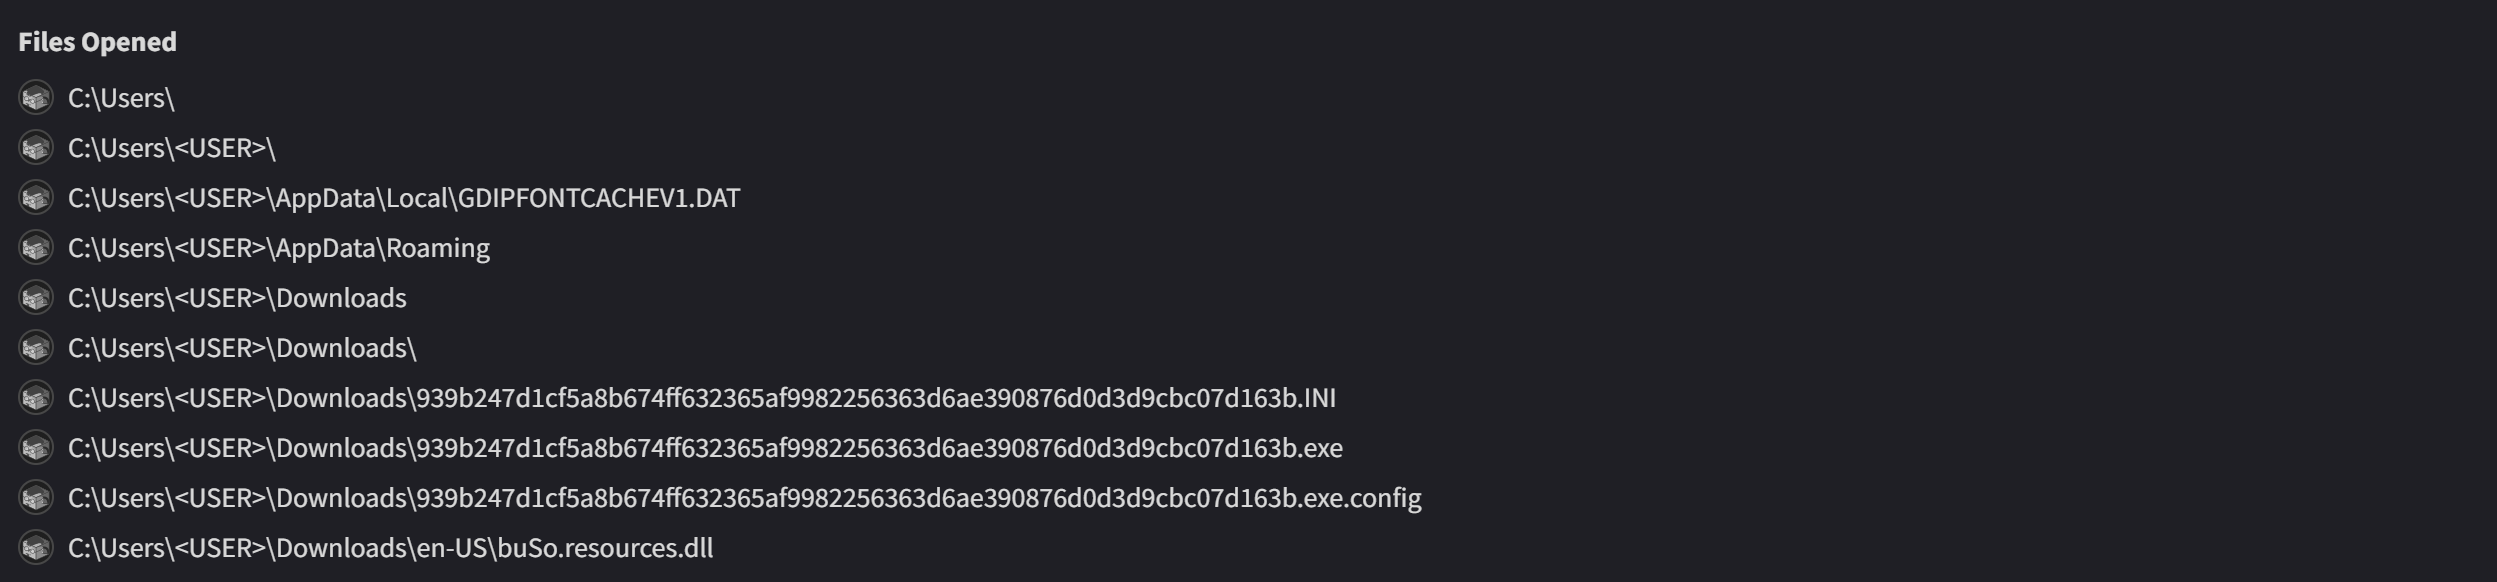
\includegraphics[width=0.75\textwidth]{images/2.3-vtdetails1.png}\\ 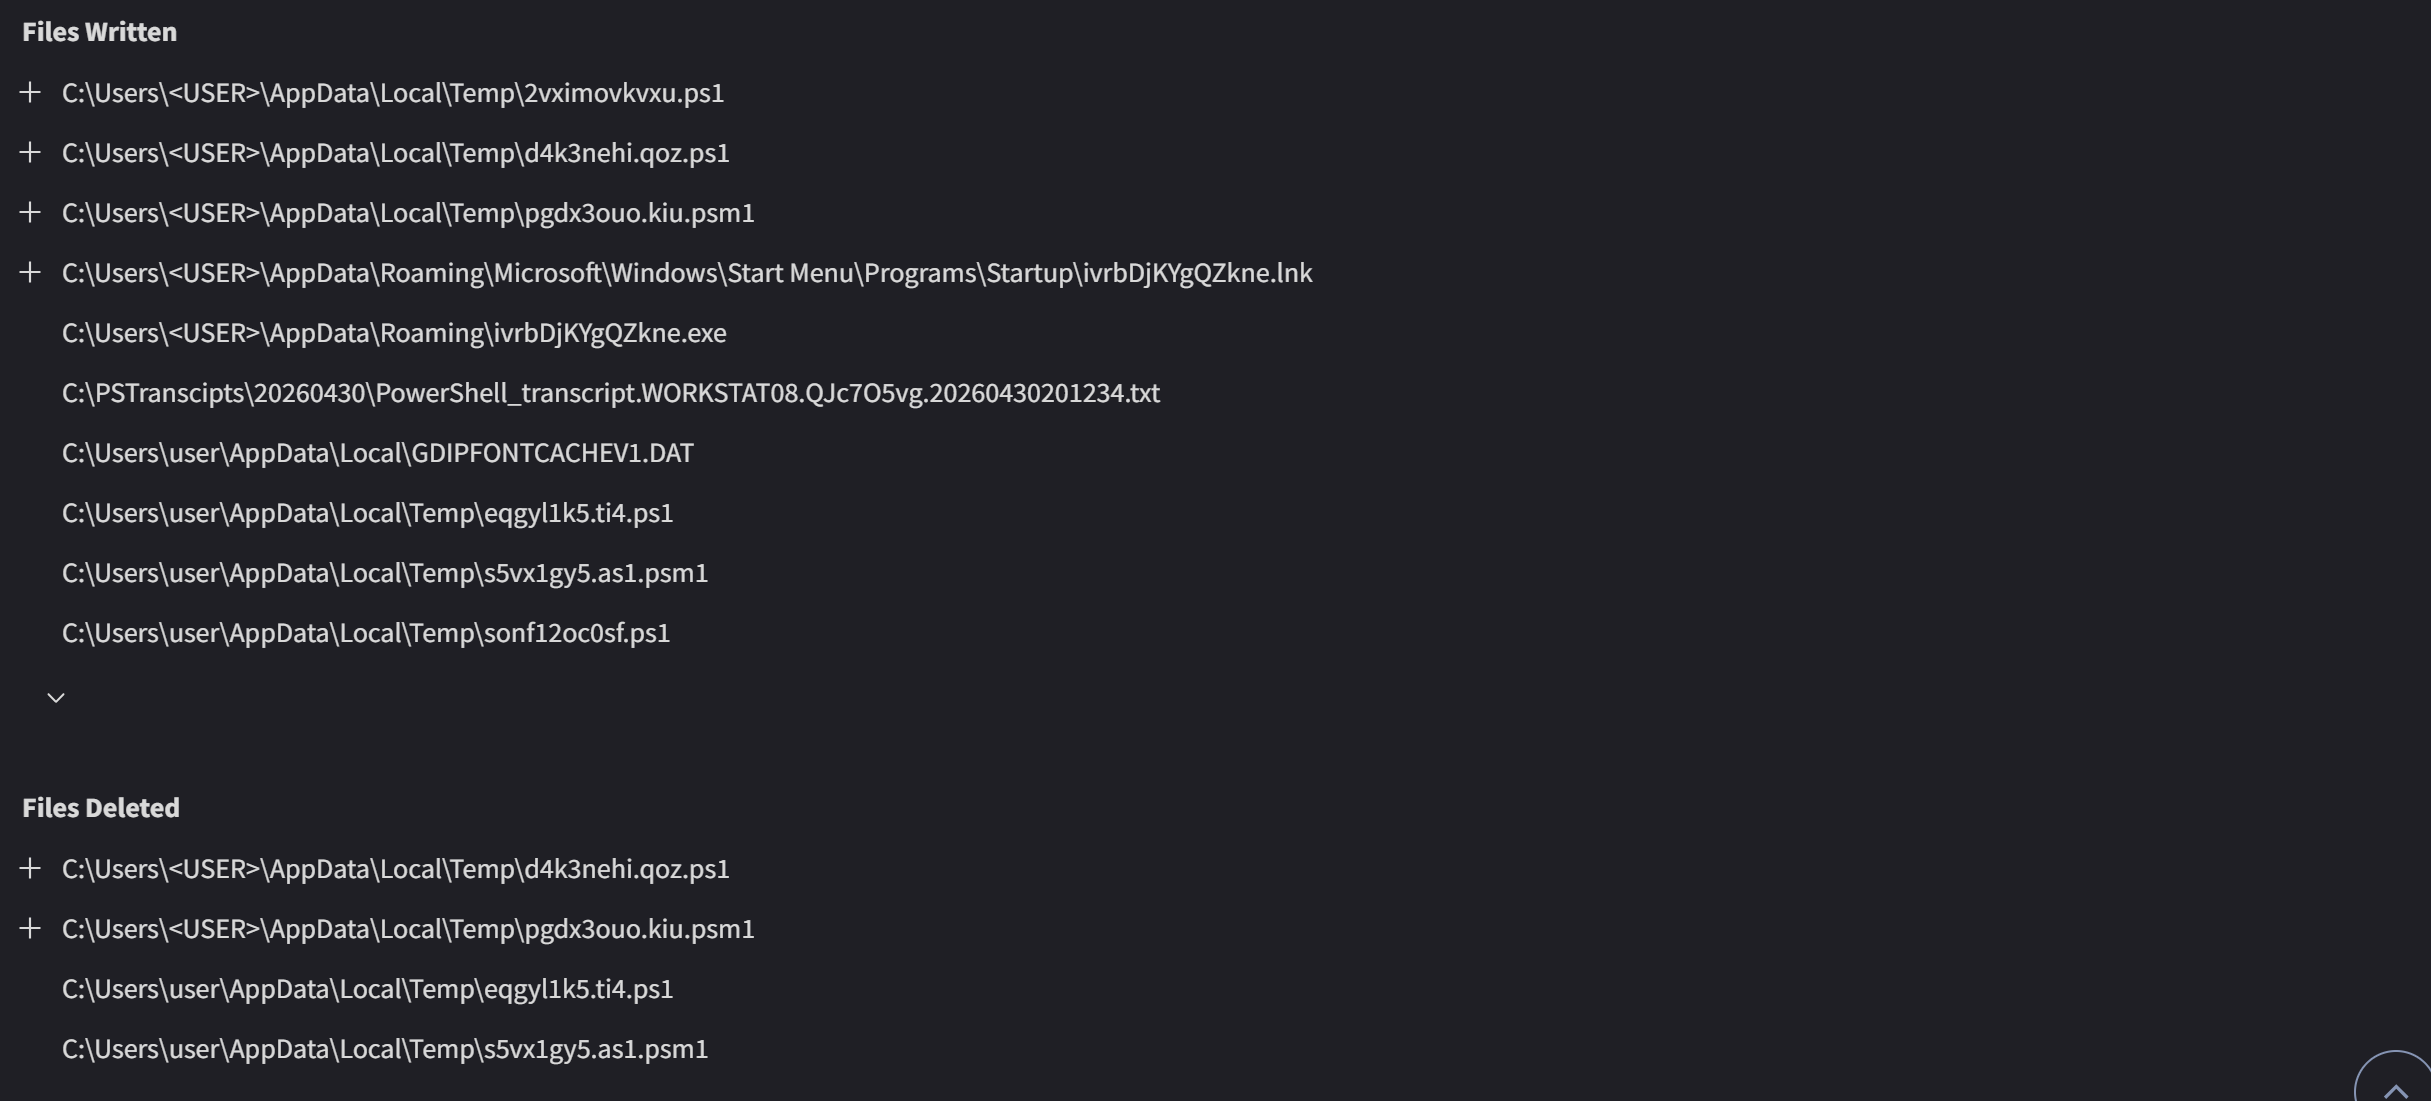
\includegraphics[width=0.75\textwidth]{images/2.4-vtdetails2.png}\\ 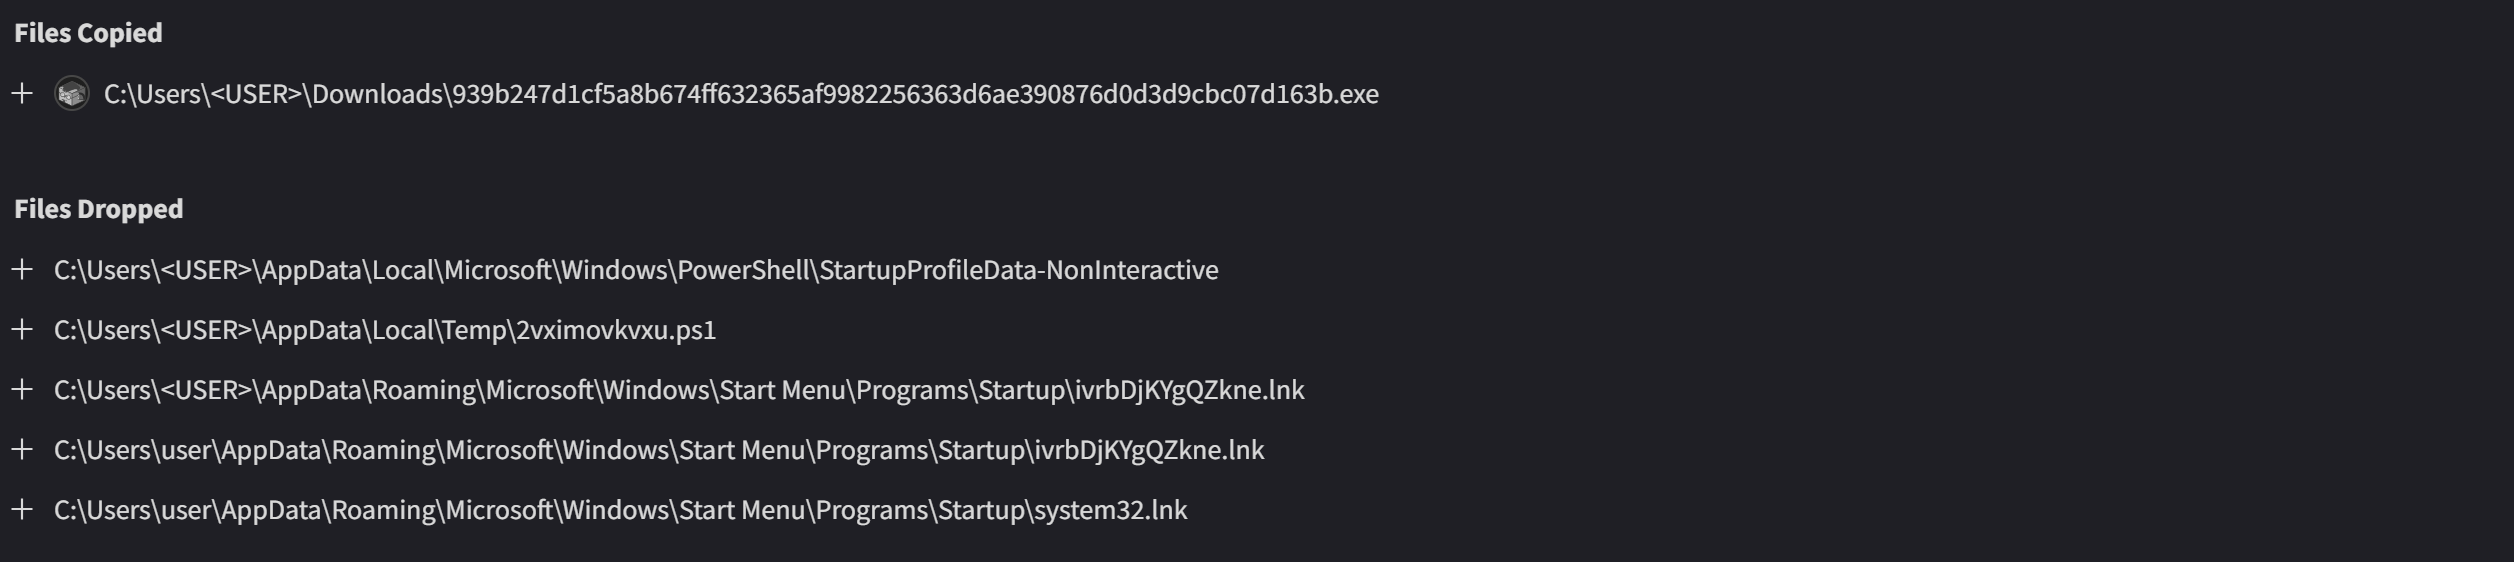
\includegraphics[width=0.75\textwidth]{images/2.5-vtdetails3.png}\\
	\textit{Figures 2.3-.5: Details of Malware file operations}
	\item \textbf{Registry Actions:}\\
	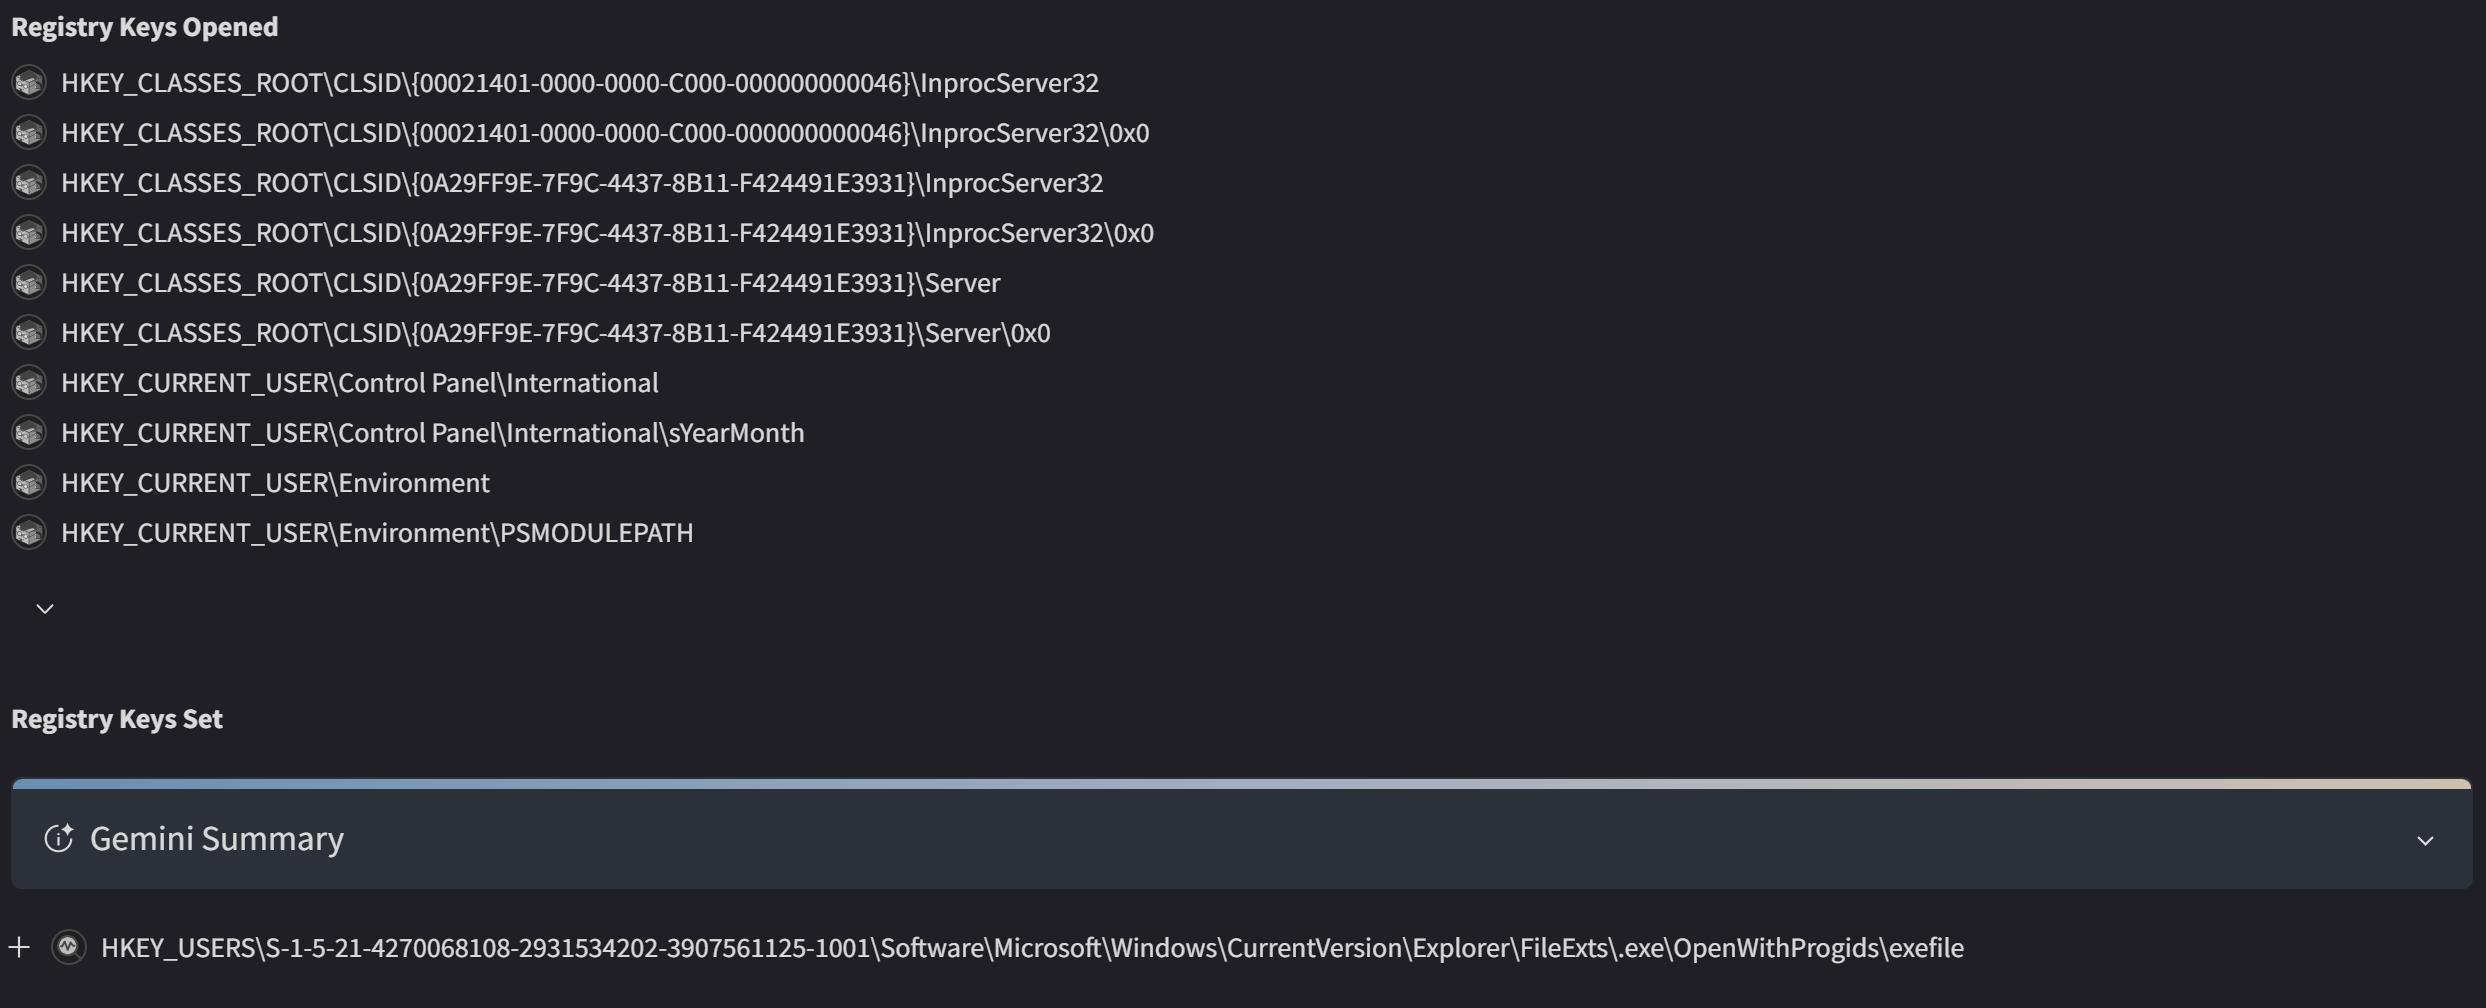
\includegraphics[width=0.75\textwidth]{images/2.6-vtdetails4.png}\\
	\textit{Figure 2.6: Details of Malware registry actions}
	\item \textbf{Network Communications}
	\begin{itemize}
		\item IP Traffic
		\begin{itemize}
			\item UDP 8.8.8.8:53
			\item TCP 199.232.210.172:80
		\end{itemize}
	\end{itemize}
	\item \textbf{MITRE ATT\&CK Techniques:}\\
	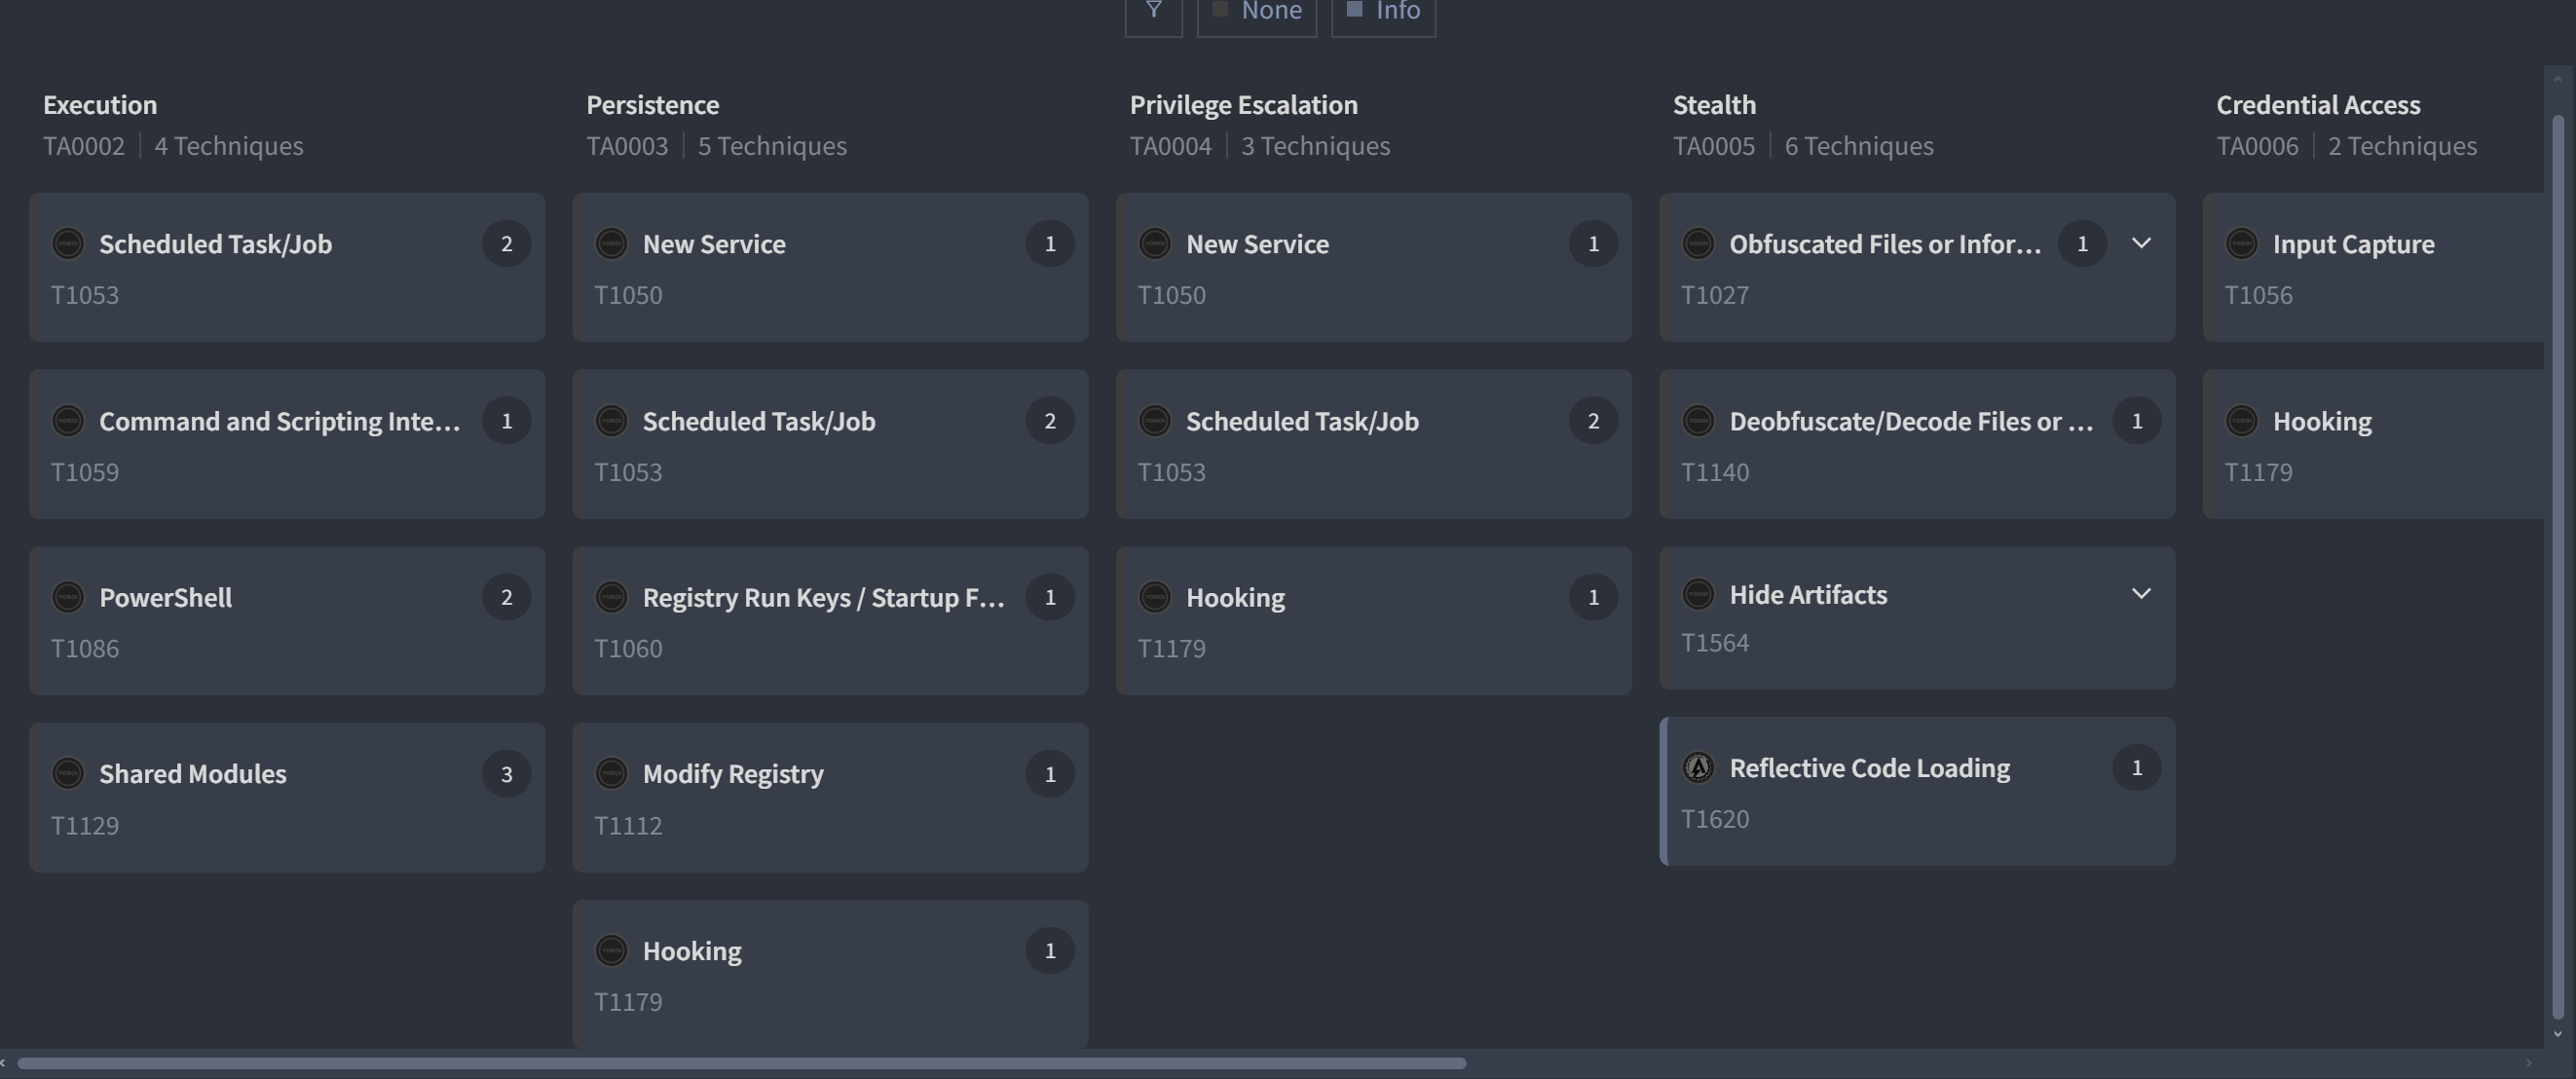
\includegraphics[width=0.75\textwidth]{images/2.7-mitretechniques.png}\\
	\textit{Figure 2.7: Table of MITRE ATT\&CK techniques used}
\end{itemize}
\textbf{Relations Tab}
\begin{itemize}
	\item \textbf{Contacted IPs:}\\
	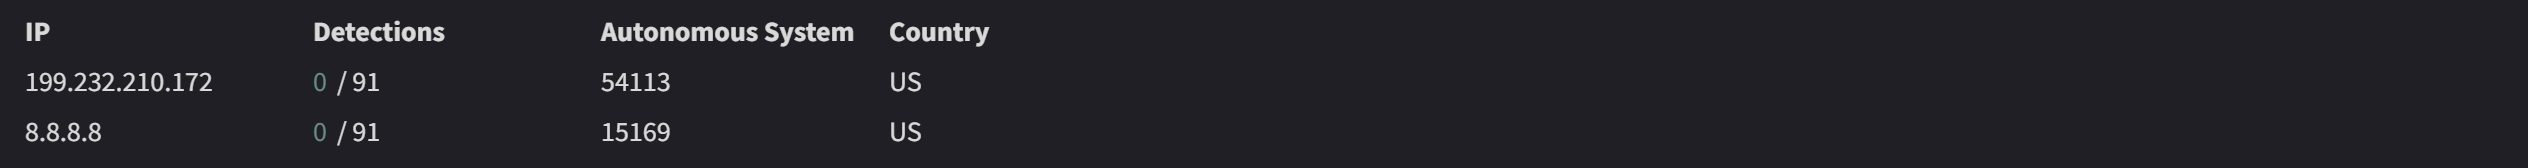
\includegraphics[width=0.75\textwidth]{images/2.8-relationsips.png}
	\item \textbf{Dropped Files:}\\
	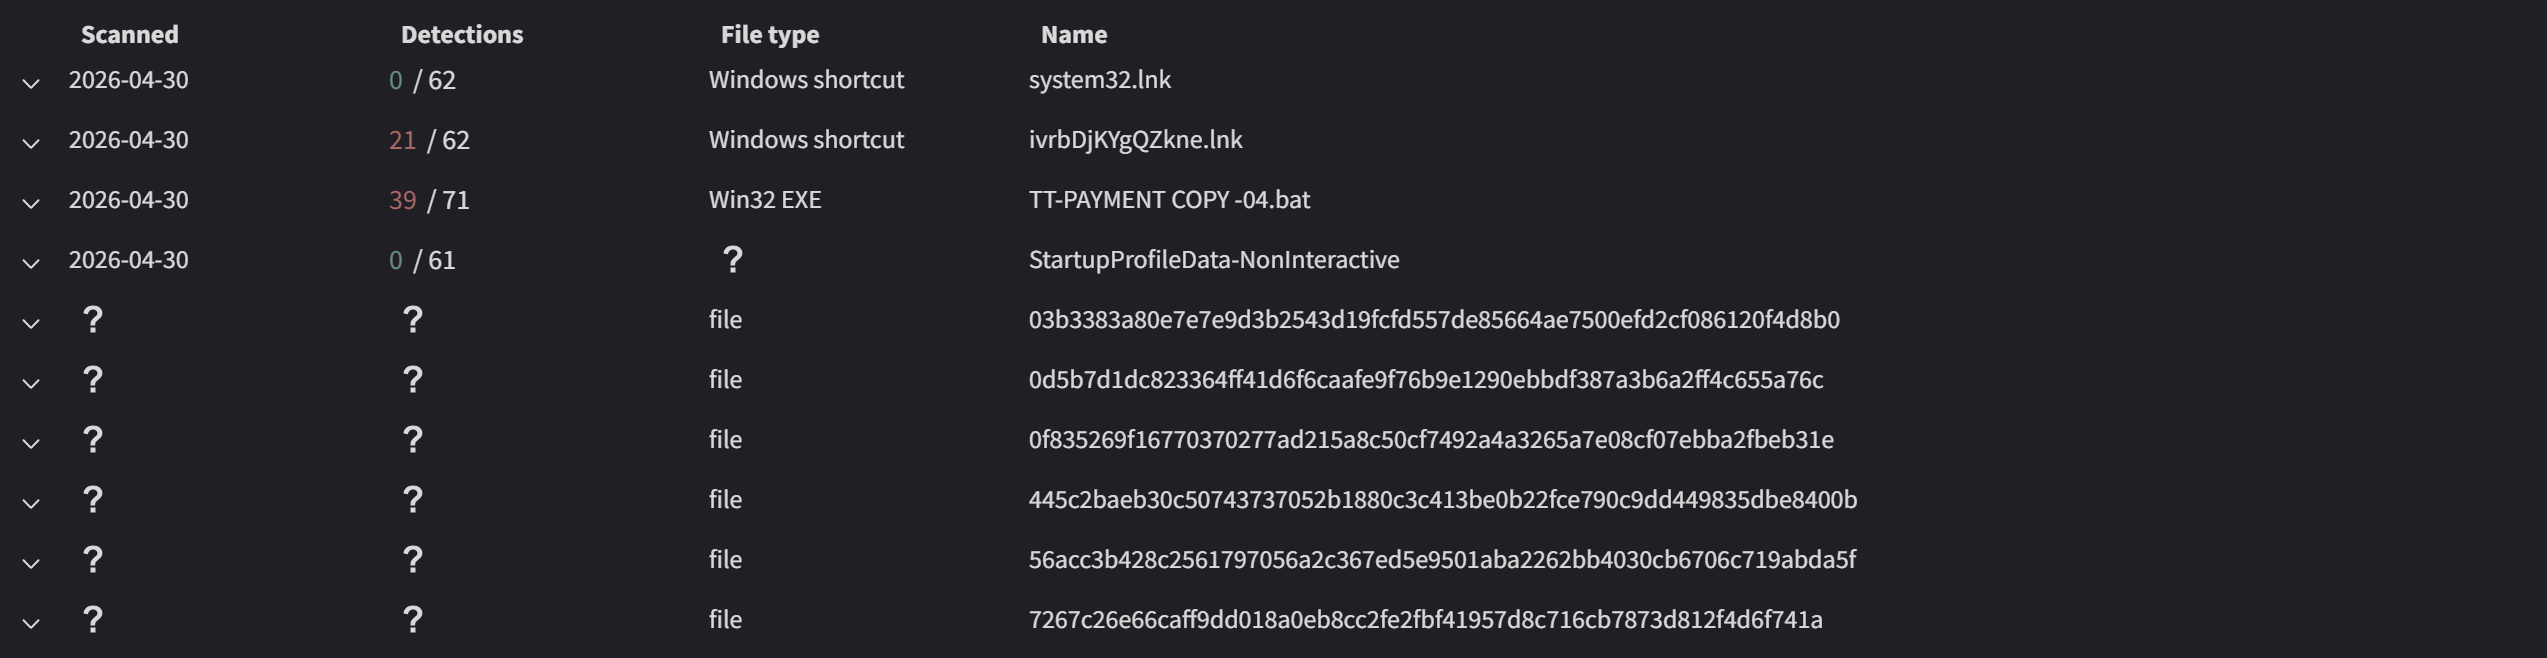
\includegraphics[width=0.75\textwidth]{images/2.9-relationsdrops.png}
	\item \textbf{Related Samples:}\\
	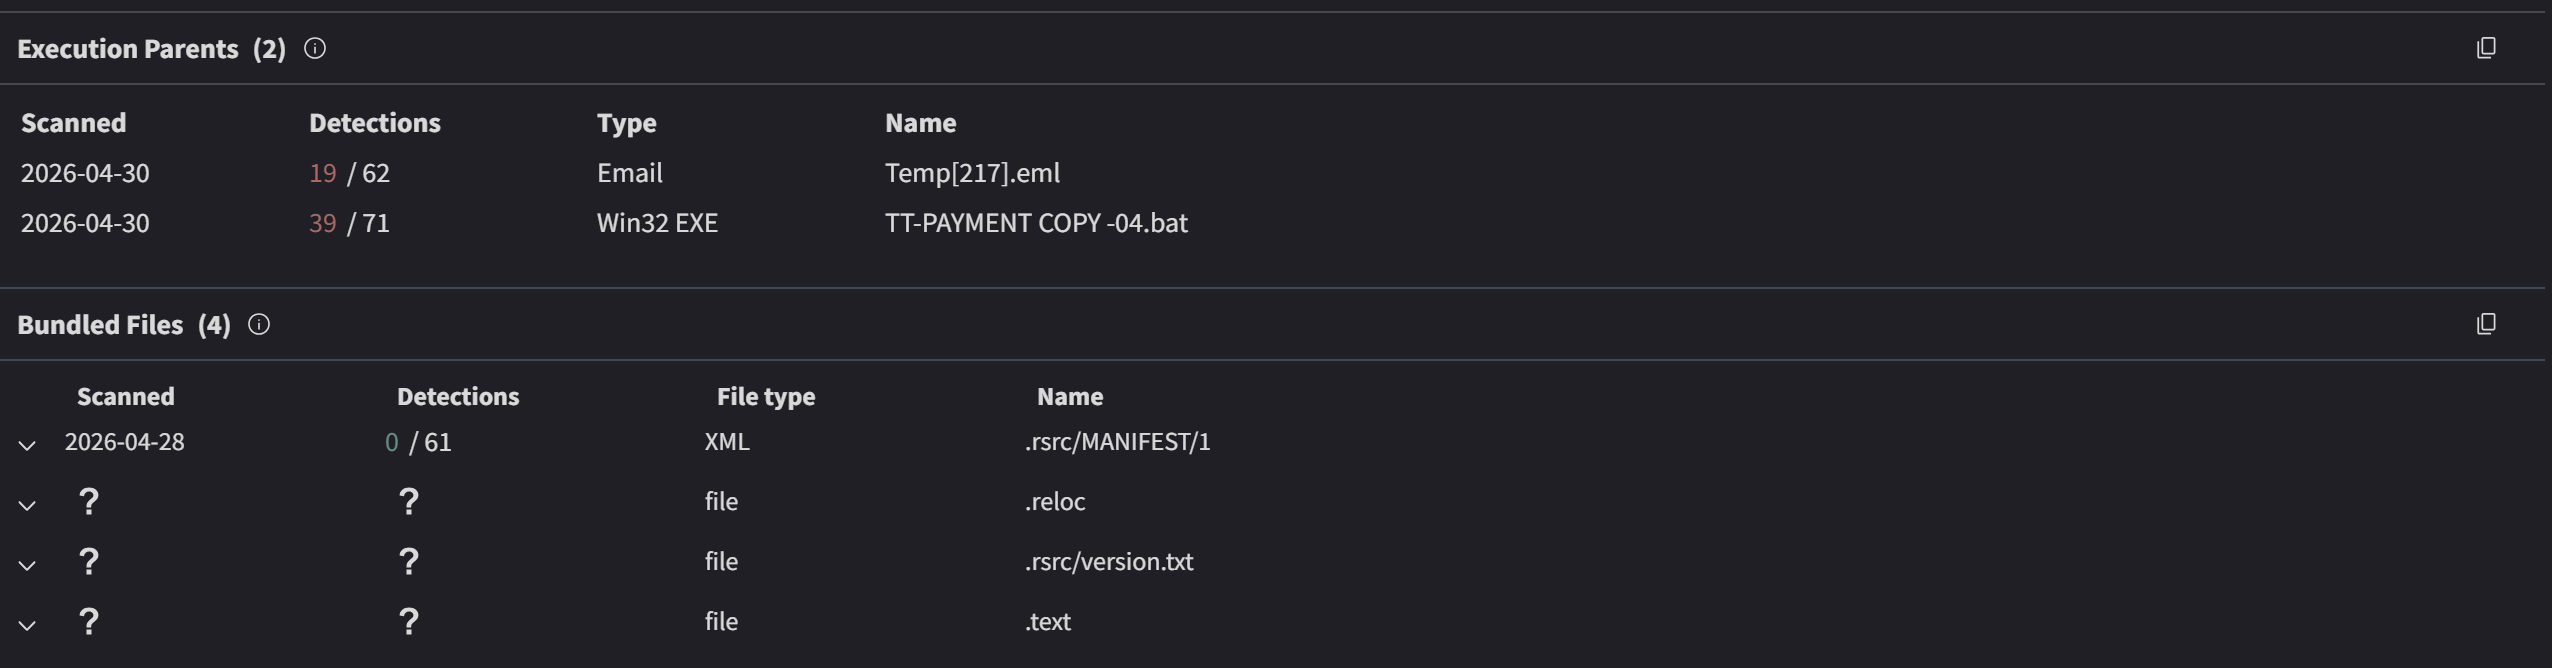
\includegraphics[width=0.75\textwidth]{images/2.10-relationsother.png}
\end{itemize}

% ++++ Part03 Dynamic Analysis ++++
\section{Dynamic Analysis}

% ++++ Part04 IOC Report & Detection ++++
\section{IOC Report \& Detection}

\vfill
\textit{++report written and formatted with help from Claude (Sonnet 4.6)++}
\end{document}

% +++++++++ Helpful stuff +++++++++++
%
% +++ Terminal-style box +++
%\begin{lstlisting}[style=terminal]
%apt-get update && apt-get install -y iptables-persistent
%\end{lstlisting}


% +++++++++ Helpful stuff +++++++++++
%
% +++ Using Minipages +++
% \begin{minipage}[t]{\linewidth}
% \includegraphics[width=0.50\textwidth]{*Image file}\\
% \textit{*Image subtitle}
% \end{minipage}
% \end{enumerate}
%

% ++++++++ Non Ticked Lists (terminal style) ++++++++++++
%\begin{lstlisting}[style=terminal]
%# Flush all existing rules
%iptables -F
%iptables -X
%iptables -t nat -F
%iptables -t nat -X
%\end{lstlisting}

%# Set default DROP on INPUT and FORWARD; OUTPUT remains ACCEPT
%iptables -P INPUT DROP
%iptables -P FORWARD DROP
%iptables -P OUTPUT ACCEPT
%\end{lstlisting}

% +++++++ Example for Using Boxes(Defined at top) +++++++++++++
%\begin{warnbox}
%\textbf{Warning:} After setting INPUT to DROP, new SSH sessions from untrusted
%interfaces will be blocked immediately. Ensure you are connected via eth0
%(management side) before proceeding, or have console access as a fallback.
%\end{warnbox}

% +++  Longtable exa,mple (with color) +++
%\noindent
%\begin{longtable}{>{\bfseries}p{0.8cm} p{2.0cm} p{5.2cm} p{1.3cm} p{1.5cm} p{2.4cm}}
%  \rowcolor{headercol}
%  \hcell{ID} & \hcell{Severity} & \hcell{Finding} &
%  \hcell{CVSS} & \hcell{Composite} & \hcell{System(s)} \\
%  \endfirsthead
%  \rowcolor{headercol}
%  \hcell{ID} & \hcell{Severity} & \hcell{Finding} &
%  \hcell{CVSS} & \hcell{Composite} & \hcell{System(s)} \\
%  \endhead
%  \midrule
%  \hline
%  F1 &
%  \sevbadge{medcol}{MEDIUM} &
%  Anonymous FTP login --- confidential directory exposed &
%  \cellcolor{lightyellow}6.4 &
%  \cellcolor{lightred}\textbf{5.00} &
%  Ubuntu (.102) \\[4pt]
% \hline
%  F2 &
%  \sevbadge{medcol}{MEDIUM} &
%  Cleartext HTTP credential transmission &
%  \cellcolor{lightyellow}4.8 &
%  \cellcolor{lightred}\textbf{4.45} &
%  Ubuntu (.102) \\[4pt]
% \hline
%  F3 &
%  \sevbadge{medcol}{MEDIUM} &
%  FTP authenticated sessions over cleartext &
%  \cellcolor{lightyellow}4.8 &
%  3.95 &
%  Ubuntu (.102) \\[4pt]
% \hline
%  FW1 &
%  \sevbadge{highcol}{HIGH{*}} &
%  Firewall default ACCEPT policy on all chains &
% \cellcolor{lightgray}N/A &
%  \cellcolor{lightgray}N/A &
%  Router (.106) \\[4pt]
% \hline
%  FW2 &
%  \sevbadge{highcol}{HIGH{*}} &
%  Unrestricted inter-zone forwarding (all ports/protocols) &
%  \cellcolor{lightgray}N/A &
%  \cellcolor{lightgray}N/A &
%  Router (.106) \\[4pt]
% \hline
%  FW3 &
%  \sevbadge{medcol}{MEDIUM} &
%  No stateful inspection --- no established/related tracking &
%  \cellcolor{lightgray}N/A &
%  \cellcolor{lightgray}N/A &
%  Router (.106) \\[4pt]
% \hline
%  FW4 &
%  \sevbadge{medcol}{MEDIUM} &
%  Management services (SSH, Webmin) exposed on all interfaces &
%  \cellcolor{lightgray}N/A &
%  \cellcolor{lightgray}N/A &
%  Router (.106) \\[4pt]
% \hline
%  F4 &
%  \sevbadge{medcol}{MEDIUM} &
%  Deprecated TLS 1.0/1.1 on RDP service &
%  \cellcolor{lightyellow}4.3 &
% 3.75 &
%  Windows (.105) \\[4pt]
% \hline
%  F5 &
%  \sevbadge{medcol}{MEDIUM} &
%  DCE/RPC endpoint enumeration --- internal service map exposed &
%  \cellcolor{lightyellow}5.0 &
%  3.45 &
%  Windows (.105) \\[4pt]
% \hline
%  F6 &
%  \sevbadge{lowcol}{LOW} &
%  Weak SSH MAC algorithms (umac-64) on both servers &
%  \cellcolor{lightgreen}2.6 &
%  2.50 &
% \hline
%  F7 &
%  \sevbadge{lowcol}{LOW} &
%  TCP timestamp information disclosure &
%  \cellcolor{lightgreen}2.6 &
%  1.95 &
%  Ubuntu, Windows \\[4pt]
% \hline
%  F8 &
%  \sevbadge{lowcol}{LOW} &
%  ICMP timestamp reply enabled &
%  \cellcolor{lightgreen}2.1 &
%  1.95 &
%  Ubuntu (.102) \\[4pt]
%  \bottomrule
%\end{longtable}